\documentclass{beamer}
\usepackage[pdftex]{graphicx}
\usepackage{multicol}
\usetheme{Malmoe}
\begin{document}
  \title{Research Knowledge Advantage Machine}
  \author{Larry Reaves\and Shifu Hao\and Chun-Wei Chiang\and Aaron Saas\and Dr. Yenumula Reddy}
  \frame{\titlepage}
  \begin{frame}
    \frametitle{Introduction}
    Research KAM is presented as a tool that helps the actual process of developing content for a paper as well as integrating a LaTeX editor for formatting.\\
    \medskip
    This tool provides an advantage for the researcher/writer of a paper by storing/indexing known knowledge points (JANs) as well as
    attempting to locate new knowledge.
  \end{frame}
  \begin{frame}
    \frametitle{Interface}
    \begin{centering}
    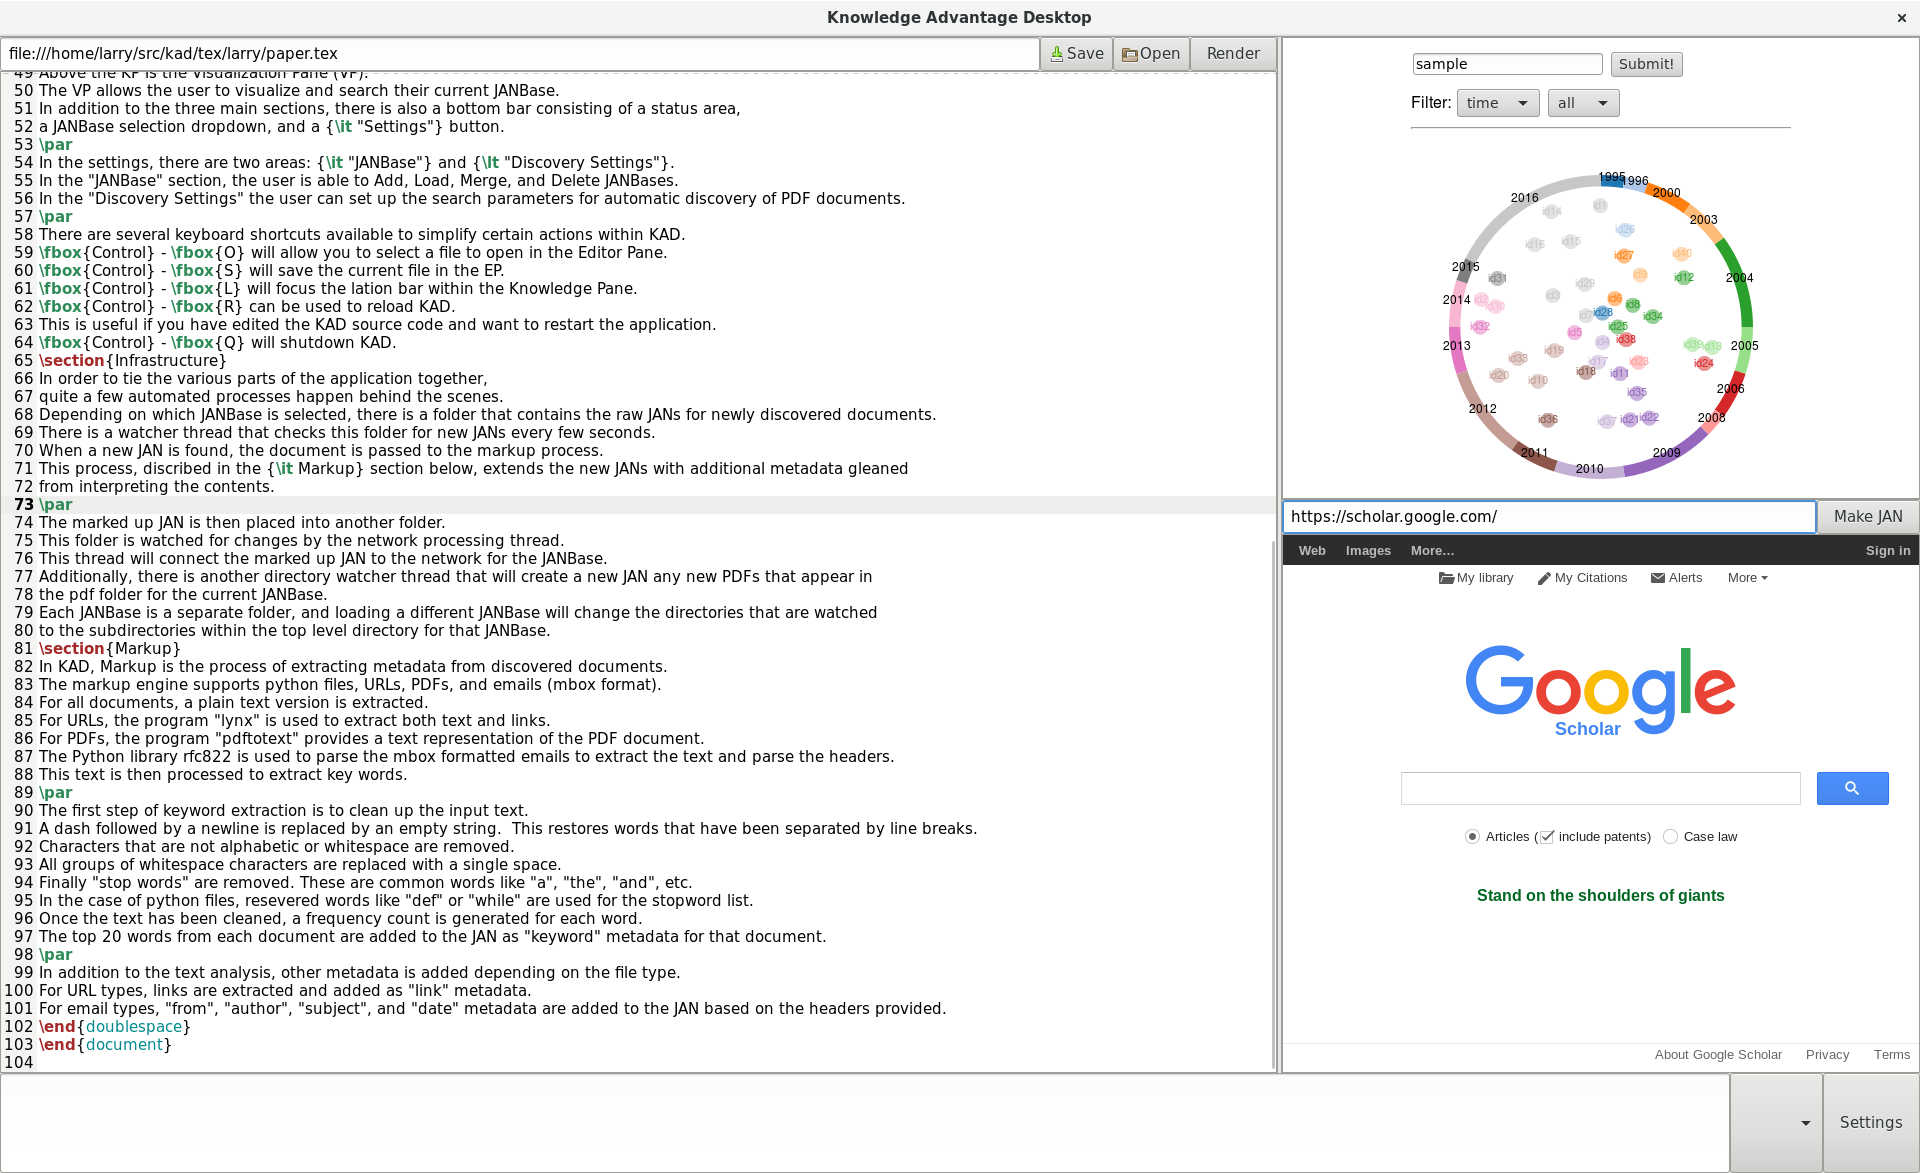
\includegraphics[width=3in]{kad-overview}\\
    \end{centering}
    The KAD interface consists of three resizable areas\\
    \begin{itemize}
    \item{Editor Pane for producing content}
    \item{Knowledge Pane for viewing URL and PDF documents}
    \item{Visualization Pane for viewing and searching the current JANBase network}
    \end{itemize}
  \end{frame}
  \begin{frame}
    \frametitle{KAM Architecture}
    A KAM typically has four main components:  Search, Markup, Network, and Visualization.\\
    \medskip
    \begin{centering}
    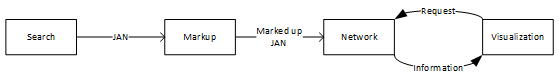
\includegraphics[width=\linewidth]{KAM}
    \end{centering}
  \end{frame}
  \begin{frame}
    \frametitle{Search}
    Search is an agent that locates JANs.  The JANs could be located in web pages, emails, pdf files, etc.\\
    \medskip
    By specifying keywords and other search parameters, existing literature will be searched and relavent PDF files downloaded.\\
    \medskip
    Manually discovered documents can also be added into the KAM with the click of a single button.
  \end{frame}
  \begin{frame}
    \frametitle{Markup}
    The software automatically annotates documents\\
    \begin{itemize}
    \item{Extracts text from PDFs, URLs, text files, emails}
    \item{Performs frequency analysis to extract the top 20 words in the text}
    \item{Extracts links from HTML documents}
    \item{Extracts headers from emails}
    \end{itemize}
  \end{frame}
  \begin{frame}
    \frametitle{Network}
    One of the major tasks of developing a KAM is creating the network that manages storing, indexing, and developing interconnectivity of JANs.\\
    \medskip
    Based upon a standard graph design, the network creates tiers of descriptors that allow quick access to nodes associated with it.\\
    \medskip
    \centering
    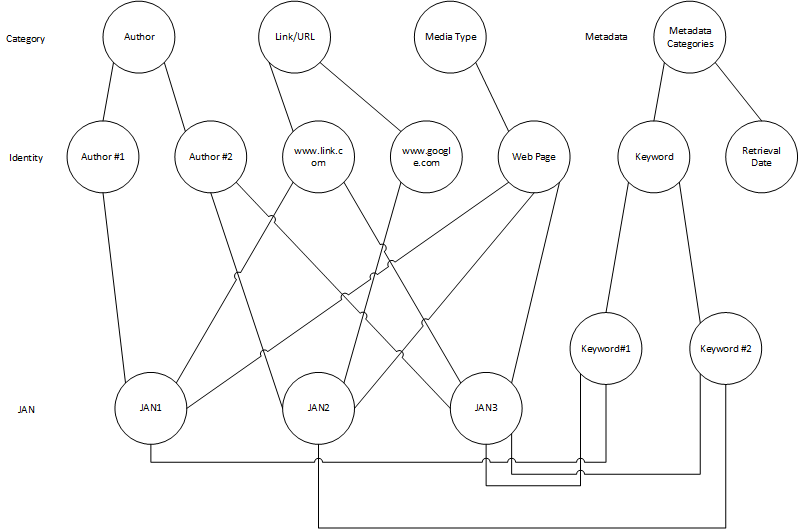
\includegraphics[width=0.5\linewidth]{Network}
  \end{frame}
  \begin{frame}
    \frametitle{Visualization}
    \begin{multicols}{2}
    Knowledge Maps are used to provide
    \begin{itemize}
    \item Knowledge management
    \item Knowledge transfer
    \item Protect against information overload
    \item Avoid misunderstanding 
    \end{itemize}
    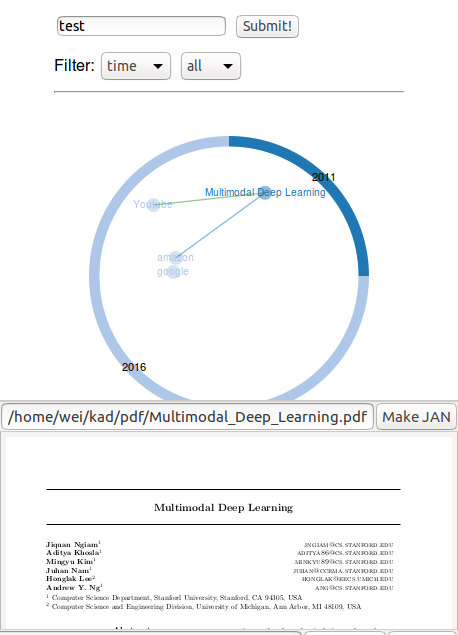
\includegraphics[width=0.9\linewidth]{fig2}
    \end{multicols}
  \end{frame}
  \begin{frame}
    \frametitle{JANBases}
    The KAM has the ability to handle multiple JANBases.\\
    \medskip
    Researchers in two different fields are not likely to be using the same information sets.\\
    \medskip
    JANBases are set up so that each group may have their own knowledge base which is specifically tailored.\\
    \medskip
    This increases the overall performance of the network by lessening memory requirements and processing.
  \end{frame}
\end{document}